\documentclass{standalone}
\usepackage{tikz}
\usetikzlibrary{patterns, positioning}

\begin{document}
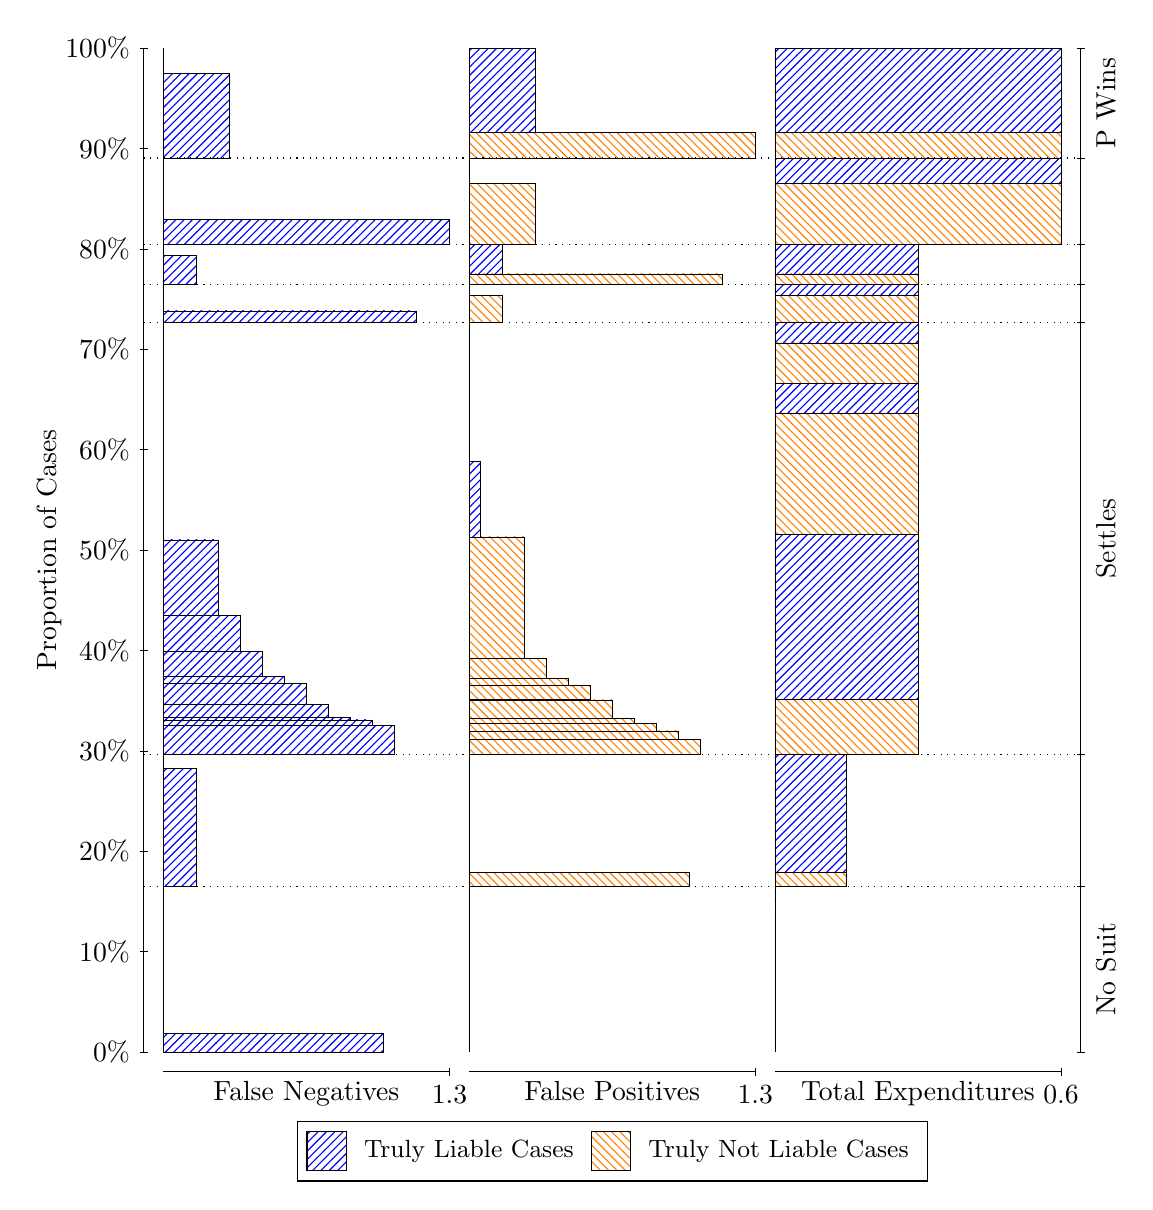
\begin{tikzpicture}
\draw[black, very thin] (1.5,1.75) -- (1.5,14.5);
\node[rotate=90, anchor=center] at (0.3, 8.125) {Proportion of Cases};
\draw[black, very thin] (1.45,1.75) -- (1.55,1.75);
\node[anchor=east] at (1.45, 1.75) {0\%};
\draw[black, very thin] (1.45,3.025) -- (1.55,3.025);
\node[anchor=east] at (1.45, 3.025) {10\%};
\draw[black, very thin] (1.45,4.3) -- (1.55,4.3);
\node[anchor=east] at (1.45, 4.3) {20\%};
\draw[black, very thin] (1.45,5.575) -- (1.55,5.575);
\node[anchor=east] at (1.45, 5.575) {30\%};
\draw[black, very thin] (1.45,6.85) -- (1.55,6.85);
\node[anchor=east] at (1.45, 6.85) {40\%};
\draw[black, very thin] (1.45,8.125) -- (1.55,8.125);
\node[anchor=east] at (1.45, 8.125) {50\%};
\draw[black, very thin] (1.45,9.4) -- (1.55,9.4);
\node[anchor=east] at (1.45, 9.4) {60\%};
\draw[black, very thin] (1.45,10.675) -- (1.55,10.675);
\node[anchor=east] at (1.45, 10.675) {70\%};
\draw[black, very thin] (1.45,11.95) -- (1.55,11.95);
\node[anchor=east] at (1.45, 11.95) {80\%};
\draw[black, very thin] (1.45,13.225) -- (1.55,13.225);
\node[anchor=east] at (1.45, 13.225) {90\%};
\draw[black, very thin] (1.45,14.5) -- (1.55,14.5);
\node[anchor=east] at (1.45, 14.5) {100\%};

\draw[black, very thin] (13.4,1.75) -- (13.4,14.5);
\draw[black, very thin] (13.35,1.75) -- (13.45,1.75);
\node[anchor=west] at (13.35, 1.75) {};
\draw[black, very thin] (13.35,3.8501) -- (13.45,3.8501);
\node[anchor=west] at (13.35, 3.8501) {};
\draw[black, very thin] (13.35,5.5297) -- (13.45,5.5297);
\node[anchor=west] at (13.35, 5.5297) {};
\draw[black, very thin] (13.35,11.015) -- (13.45,11.015);
\node[anchor=west] at (13.35, 11.015) {};
\draw[black, very thin] (13.35,11.502) -- (13.45,11.502);
\node[anchor=west] at (13.35, 11.502) {};
\draw[black, very thin] (13.35,12.002) -- (13.45,12.002);
\node[anchor=west] at (13.35, 12.002) {};
\draw[black, very thin] (13.35,13.103) -- (13.45,13.103);
\node[anchor=west] at (13.35, 13.103) {};
\draw[black, very thin] (13.35,14.5) -- (13.45,14.5);
\node[anchor=west] at (13.35, 14.5) {};

\draw[black, very thin, pattern color=blue, pattern=north east lines] (1.75,1.75) rectangle (4.5449,1.9849);
\draw[black, very thin, pattern color=orange, pattern=north west lines] (1.75,1.9849) rectangle (1.75,3.8501);
\draw[black, very thin, pattern color=blue, pattern=north east lines] (1.75,3.8501) rectangle (2.1692,5.3534);
\draw[black, very thin, pattern color=orange, pattern=north west lines] (1.75,5.3534) rectangle (1.75,5.5297);
\draw[black, very thin, pattern color=blue, pattern=north east lines] (1.75,5.5297) rectangle (4.6846,5.8997);
\draw[black, very thin, pattern color=blue, pattern=north east lines] (1.75,5.8997) rectangle (4.4051,5.9666);
\draw[black, very thin, pattern color=blue, pattern=north east lines] (1.75,5.9666) rectangle (4.1256,6.0031);
\draw[black, very thin, pattern color=blue, pattern=north east lines] (1.75,6.0031) rectangle (3.8462,6.1656);
\draw[black, very thin, pattern color=blue, pattern=north east lines] (1.75,6.1656) rectangle (3.5667,6.4291);
\draw[black, very thin, pattern color=blue, pattern=north east lines] (1.75,6.4291) rectangle (3.2872,6.5156);
\draw[black, very thin, pattern color=blue, pattern=north east lines] (1.75,6.5156) rectangle (3.0077,6.8396);
\draw[black, very thin, pattern color=blue, pattern=north east lines] (1.75,6.8396) rectangle (2.7282,7.2954);
\draw[black, very thin, pattern color=blue, pattern=north east lines] (1.75,7.2954) rectangle (2.4487,8.2542);
\draw[black, very thin, pattern color=orange, pattern=north west lines] (1.75,8.2542) rectangle (1.75,11.015);
\draw[black, very thin, pattern color=blue, pattern=north east lines] (1.75,11.015) rectangle (4.9641,11.163);
\draw[black, very thin, pattern color=orange, pattern=north west lines] (1.75,11.163) rectangle (1.75,11.502);
\draw[black, very thin, pattern color=blue, pattern=north east lines] (1.75,11.502) rectangle (2.1692,11.871);
\draw[black, very thin, pattern color=orange, pattern=north west lines] (1.75,11.871) rectangle (1.75,12.002);
\draw[black, very thin, pattern color=blue, pattern=north east lines] (1.75,12.002) rectangle (5.3833,12.326);
\draw[black, very thin, pattern color=orange, pattern=north west lines] (1.75,12.326) rectangle (1.75,13.103);
\draw[black, very thin, pattern color=blue, pattern=north east lines] (1.75,13.103) rectangle (2.5885,14.175);
\draw[black, very thin, pattern color=orange, pattern=north west lines] (1.75,14.175) rectangle (1.75,14.5);
\draw[black, very thin, pattern color=orange, pattern=north west lines] (5.6333,1.75) rectangle (5.6333,3.6152);
\draw[black, very thin, pattern color=blue, pattern=north east lines] (5.6333,3.6152) rectangle (5.6333,3.8501);
\draw[black, very thin, pattern color=orange, pattern=north west lines] (5.6333,3.8501) rectangle (8.4282,4.0264);
\draw[black, very thin, pattern color=blue, pattern=north east lines] (5.6333,4.0264) rectangle (5.6333,5.5297);
\draw[black, very thin, pattern color=orange, pattern=north west lines] (5.6333,5.5297) rectangle (8.5679,5.7221);
\draw[black, very thin, pattern color=orange, pattern=north west lines] (5.6333,5.7221) rectangle (8.2885,5.8274);
\draw[black, very thin, pattern color=orange, pattern=north west lines] (5.6333,5.8274) rectangle (8.009,5.9235);
\draw[black, very thin, pattern color=orange, pattern=north west lines] (5.6333,5.9235) rectangle (7.7295,5.9867);
\draw[black, very thin, pattern color=orange, pattern=north west lines] (5.6333,5.9867) rectangle (7.45,6.222);
\draw[black, very thin, pattern color=orange, pattern=north west lines] (5.6333,6.222) rectangle (7.1705,6.2272);
\draw[black, very thin, pattern color=orange, pattern=north west lines] (5.6333,6.2272) rectangle (7.1705,6.4071);
\draw[black, very thin, pattern color=orange, pattern=north west lines] (5.6333,6.4071) rectangle (6.891,6.4901);
\draw[black, very thin, pattern color=orange, pattern=north west lines] (5.6333,6.4901) rectangle (6.6115,6.7451);
\draw[black, very thin, pattern color=orange, pattern=north west lines] (5.6333,6.7451) rectangle (6.3321,8.2906);
\draw[black, very thin, pattern color=blue, pattern=north east lines] (5.6333,8.2906) rectangle (5.7731,9.2494);
\draw[black, very thin, pattern color=blue, pattern=north east lines] (5.6333,9.2494) rectangle (5.6333,11.015);
\draw[black, very thin, pattern color=orange, pattern=north west lines] (5.6333,11.015) rectangle (6.0526,11.354);
\draw[black, very thin, pattern color=blue, pattern=north east lines] (5.6333,11.354) rectangle (5.6333,11.502);
\draw[black, very thin, pattern color=orange, pattern=north west lines] (5.6333,11.502) rectangle (8.8474,11.633);
\draw[black, very thin, pattern color=blue, pattern=north east lines] (5.6333,11.633) rectangle (6.0526,12.002);
\draw[black, very thin, pattern color=orange, pattern=north west lines] (5.6333,12.002) rectangle (6.4718,12.78);
\draw[black, very thin, pattern color=blue, pattern=north east lines] (5.6333,12.78) rectangle (5.6333,13.103);
\draw[black, very thin, pattern color=orange, pattern=north west lines] (5.6333,13.103) rectangle (9.2667,13.428);
\draw[black, very thin, pattern color=blue, pattern=north east lines] (5.6333,13.428) rectangle (6.4718,14.5);
\draw[black, very thin, pattern color=orange, pattern=north west lines] (9.5167,1.75) rectangle (9.5167,3.6152);
\draw[black, very thin, pattern color=blue, pattern=north east lines] (9.5167,3.6152) rectangle (9.5167,3.8501);
\draw[black, very thin, pattern color=orange, pattern=north west lines] (9.5167,3.8501) rectangle (10.425,4.0264);
\draw[black, very thin, pattern color=blue, pattern=north east lines] (9.5167,4.0264) rectangle (10.425,5.5297);
\draw[black, very thin, pattern color=orange, pattern=north west lines] (9.5167,5.5297) rectangle (11.333,6.2272);
\draw[black, very thin, pattern color=blue, pattern=north east lines] (9.5167,6.2272) rectangle (11.333,8.3215);
\draw[black, very thin, pattern color=orange, pattern=north west lines] (9.5167,8.3215) rectangle (11.333,9.867);
\draw[black, very thin, pattern color=blue, pattern=north east lines] (9.5167,9.867) rectangle (11.333,10.237);
\draw[black, very thin, pattern color=orange, pattern=north west lines] (9.5167,10.237) rectangle (11.333,10.755);
\draw[black, very thin, pattern color=blue, pattern=north east lines] (9.5167,10.755) rectangle (11.333,11.015);
\draw[black, very thin, pattern color=orange, pattern=north west lines] (9.5167,11.015) rectangle (11.333,11.354);
\draw[black, very thin, pattern color=blue, pattern=north east lines] (9.5167,11.354) rectangle (11.333,11.502);
\draw[black, very thin, pattern color=orange, pattern=north west lines] (9.5167,11.502) rectangle (11.333,11.633);
\draw[black, very thin, pattern color=blue, pattern=north east lines] (9.5167,11.633) rectangle (11.333,12.002);
\draw[black, very thin, pattern color=orange, pattern=north west lines] (9.5167,12.002) rectangle (13.15,12.78);
\draw[black, very thin, pattern color=blue, pattern=north east lines] (9.5167,12.78) rectangle (13.15,13.103);
\draw[black, very thin, pattern color=orange, pattern=north west lines] (9.5167,13.103) rectangle (13.15,13.428);
\draw[black, very thin, pattern color=blue, pattern=north east lines] (9.5167,13.428) rectangle (13.15,14.5);
\draw[black, dotted] (1.5,3.8501) -- (13.4,3.8501);
\draw[black, dotted] (1.5,5.5297) -- (13.4,5.5297);
\draw[black, dotted] (1.5,11.015) -- (13.4,11.015);
\draw[black, dotted] (1.5,11.502) -- (13.4,11.502);
\draw[black, dotted] (1.5,12.002) -- (13.4,12.002);
\draw[black, dotted] (1.5,13.103) -- (13.4,13.103);
\draw[black, very thin] (1.75,1.5) -- (5.3833,1.5);
\node[anchor=north] at (3.5667, 1.5) {False Negatives};
\draw[black, very thin] (5.3833,1.45) -- (5.3833,1.55);
\node[anchor=north] at (5.3833, 1.45) {1.3};

\draw[black, very thin] (5.6333,1.5) -- (9.2667,1.5);
\node[anchor=north] at (7.45, 1.5) {False Positives};
\draw[black, very thin] (9.2667,1.45) -- (9.2667,1.55);
\node[anchor=north] at (9.2667, 1.45) {1.3};

\draw[black, very thin] (9.5167,1.5) -- (13.15,1.5);
\node[anchor=north] at (11.333, 1.5) {Total Expenditures};
\draw[black, very thin] (13.15,1.45) -- (13.15,1.55);
\node[anchor=north] at (13.15, 1.45) {0.6};

\node[black, centered, rotate=90] at (13.72, 2.8) {No Suit};

\node[black, centered, rotate=90] at (13.72, 8.2724) {Settles};



\node[black, centered, rotate=90] at (13.72, 13.802) {P Wins};

\draw (7.449999999999999,1.5) node[draw=none] (baseCoordinate) {};
\begin{scope}[align=center]
        \matrix[scale=0.5, draw=black, below=0.5cm of baseCoordinate, nodes={draw}, column sep=0.1cm]{
            \node[rectangle, draw, minimum width=0.5cm, minimum height=0.5cm, pattern=north east lines, pattern color=blue] {}; &
            \node[draw=none, font=\small] (B) {Truly Liable Cases}; &
            \node[rectangle, draw, minimum width=0.5cm, minimum height=0.5cm, pattern=north west lines, pattern color=orange] {}; &
            \node[draw=none, font=\small] (B) {Truly Not Liable Cases}; \\
            };
\end{scope}

\end{tikzpicture}
\end{document}